\documentclass{article}

% if you need to pass options to natbib, use, e.g.:
%     \PassOptionsToPackage{numbers, compress}{natbib}
% before loading neurips_2020

% ready for submission
% \usepackage{neurips_2020}

% to compile a preprint version, e.g., for submission to arXiv, add add the
% [preprint] option:
%     \usepackage[preprint]{neurips_2020}

% to compile a camera-ready version, add the [final] option, e.g.:
%     \usepackage[final]{neurips_2020}

% to avoid loading the natbib package, add option nonatbib:

\usepackage[nonatbib]{neurips_2020}
%\usepackage[final]{neurips_2020}

\usepackage[utf8]{inputenc} % allow utf-8 input
\usepackage[T1]{fontenc}    % use 8-bit T1 fonts
\usepackage{hyperref}       % hyperlinks
\usepackage{url}            % simple URL typesetting
\usepackage{booktabs}       % professional-quality tables
\usepackage{amsfonts}       % blackboard math symbols
\usepackage{nicefrac}       % compact symbols for 1/2, etc.
\usepackage{microtype}      % microtypography
\usepackage{graphicx}

\title{Handwritten Digit Recognition on the MNIST Dataset}

% The \author macro works with any number of authors. There are two commands
% used to separate the names and addresses of multiple authors: \And and \AND.
%
% Using \And between authors leaves it to LaTeX to determine where to break the
% lines. Using \AND forces a line break at that point. So, if LaTeX puts 3 of 4
% authors names on the first line, and the last on the second line, try using
% \AND instead of \And before the third author name.

\author{%
  Tianbo Yang  \\
  Department of Computer Science\\
  Haverford College\\
  Haverford, PA  \\
  \texttt{tyang3@haverford.edu} \\
  % examples of more authors
  % \And
  % Coauthor \\
  % Affiliation \\
  % Address \\
  % \texttt{email} \\
  % \AND
  % Coauthor \\
  % Affiliation \\
  % Address \\
  % \texttt{email} \\
  % \And
  % Coauthor \\
  % Affiliation \\
  % Address \\
  % \texttt{email} \\
  % \And
  % Coauthor \\
  % Affiliation \\
  % Address \\
  % \texttt{email} \\
}

\begin{document}

\maketitle


\begin{abstract}
  In this project, we train multilayer perceptions and convolutional neural networks to classify handwritten digit images in the MNIST dataset with 10 different labels from 0 to 9. We construct a total of four neural network classifiers. The first has no hidden layers (termed ``simple perceptron"), the second has one hidden fully connected layer followed by a ReLU nonlinear function (``perceptron with ReLU"), the third has one hidden convolutional layer followed by a maximum pooling nonlinear function (``CNN"), and the fourth has two hidden layers (both one hidden convolutional layer with a maximum pooling function and one hidden fully connected layer with a ReLU function)(``CNN with ReLU"). We use the standard negative log-likelihood loss function and the Adam optimizer in this project as it outperforms other options. Finally, we compare the performances of the four models, analyze their weaknesses, and use the Bayesian analytical framework to find how confident the models are for any predicted value.
\end{abstract}

\section{Introduction}

%NeurIPS requires electronic submissions.  The electronic submission site is
%\begin{center}
%  \url{https://cmt3.research.microsoft.com/NeurIPS2020/}
%\end{center}

Handwritten digit classification is a standard problem in computer vision and deep learning. It is involved in real life applications such as recognizing numbers on checks, street signs, license plates, etc. Scientists and engineers with interests in image processing and pattern recognition have developed various approaches to solve this problem ([2], [3], and [5]). These include multilayer perceptions (MLPs) and convolutional neural networks (CNNs). Although these technologies have matured over the decades with respect to improving predictive accuracy, it is nevertheless insightful to compare the strengths and weaknesses of different types of classifiers and identify the design choices that give rise to them. For example, convolutional layers are designed to detect local features such as edges so that objects do not have to be centered in the image. They are usually used with nonlinear maximum pooling functions to greatly increase the predictive accuracy. We are also interested in the effect of adding rectified linear unit (ReLU) funtions to perceptrons and CNNs. Some features that a linear classifier tends to struggle with can be mitigated by ReLU functions since they allow the data to be classified using multiple linear planes.

In this project, we use the MNIST dataset (see [4] and [1]) of handwritten digits to train four neural network classification models. The first model is a simple perceptron with a 10-way softmax output layer. Then we add a hidden fully connected layer with a ReLU nonlinear function to the first one to form the second model. In the third model, instead of adding ReLU functions, we add a hidden convolutional layer with a maximum pooling nonlinear function to the first model to set up a simple convolutional neural network. Finally, we construct a complex neural network by combining both hidden layers together (one convolutional layer with a maximum pooling function and one fully connected layer with a ReLU function). Throughout this project, we use the negative log-likelihood loss function to measure how bad a model's prediction is and the Adam optimizer to update network weights based on training data.  We compare the effectiveness of all models and identify the common features that the classifiers tend to struggle more with. In the end, we use Baysian analysis to find the confidence levels of each model for any given predicted outcome.

We hypothesize that adding fully connected layers with nonlinear ReLU functions to a simple perceptron greatly improves the prediction accuracy. We also expect the perceptrons and CNNs to each come with a very different set of weaknesses. The neural networks perform the best when we combine both types of layers together.

\section{Archtecture}

The MNIST dataset  contains 70,000 images. Each image has 28 $\times$ 28 pixels ($28\times 28$ matrices) in gray scale with intensity values from 0 to 255, and each is labelled by a number from 0 to 9, indicating the corresponding digit number.

\subsection{A simple perceptron with softmax output}

A perceptron is a linear map $\phi$ from $\mathbb{R}^{d} \to \mathbb{R}^n$ defined by
$$
Z=\phi(X) = WX  + B \in \mathbb{R}^n,
$$
where $X\in \mathbb{R}^{d}$ is a feature vector, $W\in \mathbb{R}^{n\times d}$ is a weight matrix, $B\in \mathbb{R}^n$ is a bias vector, and $Z\in \mathbb{R}^n$ is an output vector.

Since we have multiple classes (10 digits), we use a softmax function as the output layer. A softmax function maps $Z\in\mathbb{R}^{n} \to A\in [0, 1]^{n}$ \, with \, $\sum_{i=1}^{n} a_i=1$ by
$$
A={\rm softmax}(Z)=\left[\begin{array}{c} \frac{{\rm exp}(z_1)}{\sum_{i=1}^n {\rm exp}(z_i)}\\ \vdots\\ \frac{{\rm exp}(z_n)}{\sum_{i=1}^n {\rm exp}(z_i)}\end{array}\right].
$$
It produces a probability distribution over the $n$ class labels. We use the arg max function to generate the class label, where
$$
{\rm arg\,max}(A)=j \quad {\rm where} \quad a_{j}={\rm max}_{1\leq i\leq n}\{a_{1}, \,\dots , \,a_{n}\}.
$$
For example, in this encoding, we have ${\rm arg\,max} \left(\left[\begin{array}{ccc}1&2&5\end{array}\right]^T\right)
=3$ since the third argument has the maximum value.

In our project, we have $d=28\times 28=784$ and $n=10$. Our first model is a linear classifier that inputs an image in $\mathbb{R}^{784}$ and outputs an integer $i$, where $0\leq i\leq 9$, via the following diagram:
$$
\mathbb{R}^{784} \stackrel{\,\,\phi\,\,}{\longrightarrow} \mathbb{R}^{10}
\stackrel{\rm softmax}{\longrightarrow}\mathbb{R}^{10}\stackrel{\rm arg\,max}{\longrightarrow} i\in \{0, 1, \ldots, 9\}.
$$
To feed the data into this model, we need to flatten the images ($28\times 28$ matrices) into column vectors of size $784\times 1$.

\subsection{A perceptron with ReLU and softmax output} The ReLU function maps $\mathbb{R} \to \mathbb{R}$ by
${\rm ReLU}(z)={\rm max}\{0, z\}$. 
Observe ReLU is a nonlinear function. By dropping negative numbers, it allows multiple linear planes to classify the data.
In the second model, we add a hidden ReLU layer with 64 units as shown in the following diagram:
$$
\mathbb{R}^{784} \stackrel{\,\,\phi_1\,\,}{\longrightarrow} \mathbb{R}^{64} \stackrel{\rm ReLU}{\longrightarrow} \mathbb{R}^{64} \stackrel{\,\,\phi_2\,\,}{\longrightarrow} \mathbb{R}^{10} \stackrel{\rm softmax}{\longrightarrow}\mathbb{R}^{10}
\stackrel{\rm arg\,max}{\longrightarrow} i\in \{0, 1, \ldots, 9\}.
$$
The hidden layer is applied to all pixel values in training images, so it is called a fully connected layer.

\subsection{A perceptron with CNN and softmax output} In convolutional neural networks, small vectors (for 1D images) or matrices (for 2D images) are used to create new images. These small vectors and matrices are called filters. The filters are applied to a local spatial neighborhood of pixel values to detect the presence of some pattern in that data. It is ``tuned" to produce a high value for certain kinds of patterns/features (such as edges). This allows us to only focus on part of the image instead of the whole image. In order to detect the patterns/features anywhere in the (large) input image, we slide the filters over the image and produce a new feature map.

Convolutional layers are specified by their dimensions, sizes, and units (number of filters used). For example, conv2D(64, (3, 3)) means a convolutional layer with 64 filters, each is a small matrix of size $3\times 3$ in a 2-dimensional image. In general, the output of a convolutional layer is feeded into a maximum pooling layer to detect the largest value in every small neighborhood. After we are done with the convolutional layers, we flatten all the resulting images from pooled feature maps down to a single long linear vector and feed it into a final fully connected layer, leading into an activation function such as softmax that produces the final output.

Thus, the third model is a simple convolutional neural network constructed by adding a hidden convolutional layer with 64 units to the first model, as shown in the following diagram:
$$
\mathbb{R}^{784} \stackrel{{\rm conv2D}(64, (3, 3))}{\longrightarrow}\mathbb{R}^{784\times 64} \stackrel{\rm max \,\, pooling (2, 2)}{\longrightarrow} \mathbb{R}^{196\times 64} \stackrel{\,\,\phi\,\,}{\longrightarrow} \mathbb{R}^{10} \stackrel{\rm softmax}{\longrightarrow}\mathbb{R}^{10}\stackrel{\rm arg\,max}{\longrightarrow} i\in \{0, 1, \ldots, 9\}.
$$

\subsection{A perceptron with CNN, ReLU, and softmax output}
The fourth model is a more complicated convolutional neural network obtained by adding a ReLU layer after the convolutional layer in the third model, shown in the following diagram:
$$
\mathbb{R}^{784} \stackrel{{\rm conv2D}(64, (3, 3))}{\longrightarrow} \mathbb{R}^{784\times 64}\stackrel{\rm max\,\, pooling (2, 2)}{\longrightarrow} \mathbb{R}^{196\times 64}\stackrel{{\rm flatten}}{\longrightarrow} \mathbb{R}^{12544}
$$
$$\stackrel{\,\,\phi_1\,\,}{\longrightarrow} \mathbb{R}^{64}\stackrel{{\rm relu}(64, (3, 3))}{\longrightarrow} \mathbb{R}^{64}\stackrel{\,\,\phi_2\,\,}{\longrightarrow} \mathbb{R}^{10} \stackrel{\rm softmax}{\longrightarrow}\mathbb{R}^{10}\stackrel{\rm arg\,max}{\longrightarrow} i\in \{0, 1, \ldots, 9\}.
$$

In general, we can add a ReLU layer right after a filter layer. There maybe be multiple filter/ReLU layers, then a maximum pooling layer, then some more filter/ReLU layers, followed by another maximum pooling layer. After these layers, there is typically a last fully connected layer, leading into an activation function such as softmax that produces the final output. The exact design of these structures is an art as there is currently no clear theoretical and empirical understanding of how these various design choices affect the overall performance of the network.

\section{Implementation}

\subsection{Dataset}

We first load the MNIST dataset from TensorFlow Datasets and divide the 70,000 images into 50,000 training images, 10, 000 validation images, and 10, 000 testing images. The validation set can be used to gauge the model's generalizability during training so that the test set can serve as a final unbiased estimator for the model's performance. Before we apply a perceptron learning algorithm, we flatten all images ($28\times 28$ pixels) into column vectors of $784$ pixel numbers. Then we normalize the pixel values by dividing each by 255 so that they range from 0 to 1. This step ensures that the input pixels have similar distributions and helps with training convergence. We also convert the labels into 10-dimensional column vectors using one-hot encoding. For example, the number 5 is converted into $\left[\begin{array}{cccccccccc} 0&0&0&0&0&1&0&0&0&0\end{array}\right]^T$.

\subsection{Initialization}
We initialize the weights for each layer from a Gaussian distribution with mean 0 and standard deviation 0.01. The biases are initialized with zeros. We assign random weights to weight matrices and filters before starting the algorithm.

\subsection{Procedure}

We first find the preactivation rates and activation rates in the hidden layers using the input data, the weight matrices and/or filters, the ReLU functions and the maximum pooling functions.  Then we compute the error rate at the output layer using the negative log-likelihood loss function and feed this loss backward through the neural network layers to compute the gradient of the loss function with respect to the weights. We train and update the weights using the Adam optimizer with a minibatch of 128 images. After this, we repeat the process until the convergence criterion is met. Then we score the activation rate of the output layer using the final updated weights.

%To combat with overfitting problem, we use a recently proposed regularization technique, called Dropout. In short, it keeps a neuron unit active with some probability $p$, which is a hyperparameter. Alternatively, it can also be viewed as sampling a neural network from the full neural network where the parameter updates only contribute to the sampled neural network.

\section{Comparison of Different Classifiers}

The following graphs display performances of the four different classifiers: a simple perceptron, a perceptron with ReLU, a CNN, and a CNN with ReLU. The upper plots show the evolutions of training and validation accuracies under different models over epochs. The lower plots indicate the evolutions of the training loss and validation loss of these models over epochs.
\smallskip

\hspace{-0.3in}
\begin{minipage}{0.52\linewidth}
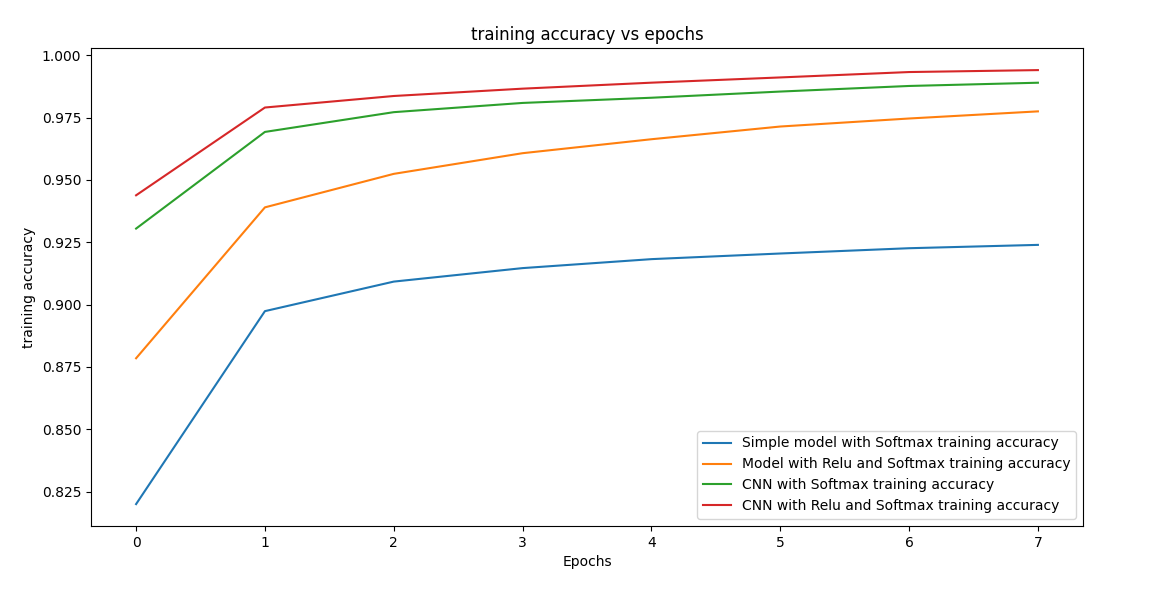
\includegraphics[width = \linewidth]{Training_accuracy.png}
\end{minipage}
\begin{minipage}{0.52\linewidth}
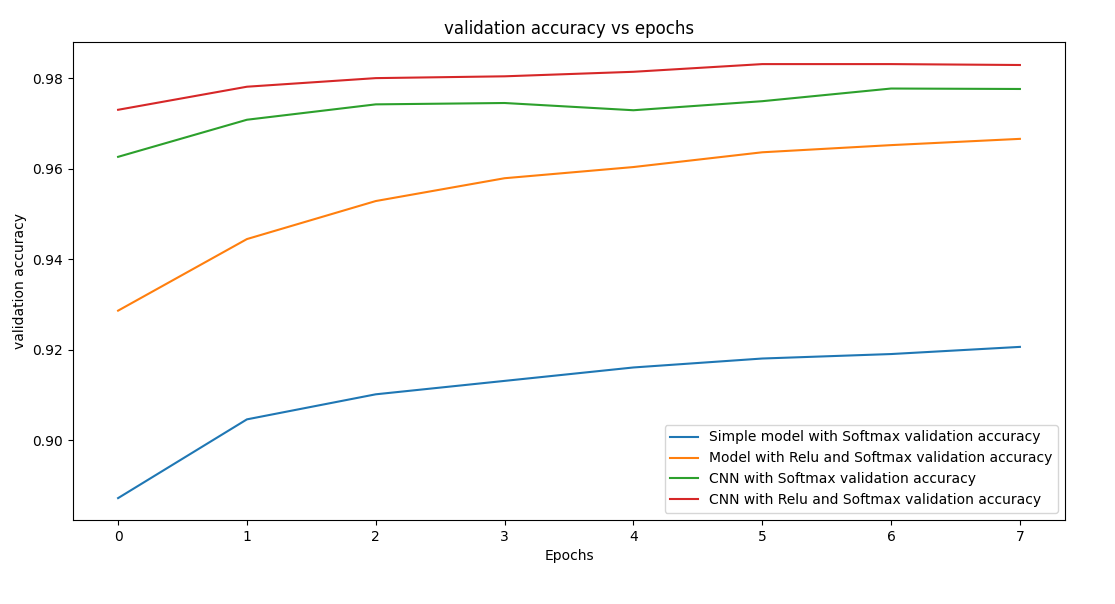
\includegraphics[width = \linewidth]{Validation_accuracy.png}
\end{minipage}

\hspace{-0.3in}
\begin{minipage}{0.52\linewidth}
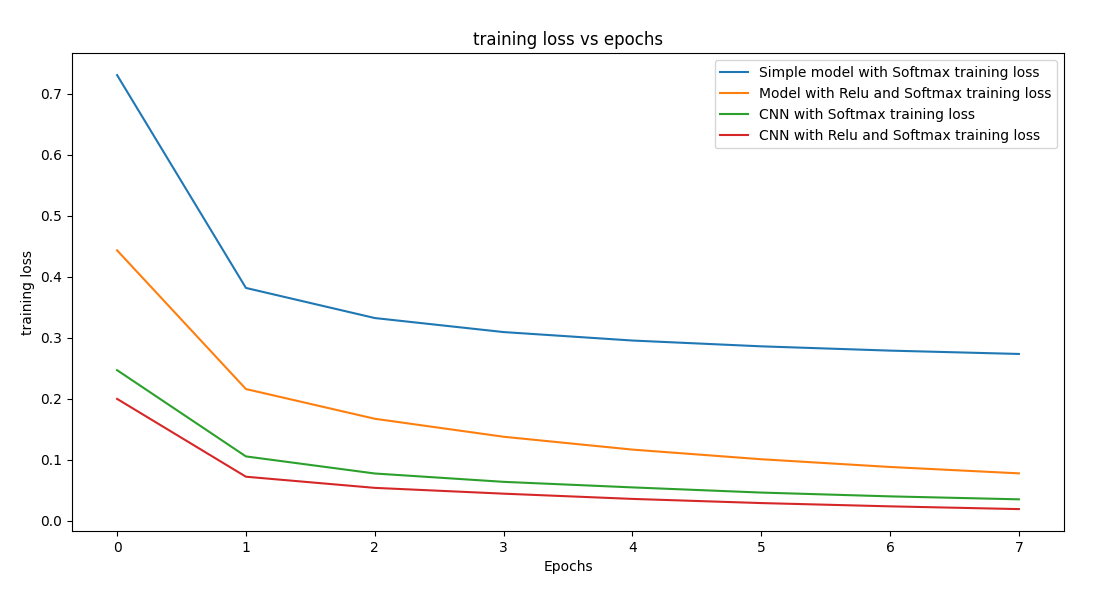
\includegraphics[width = \linewidth]{Training_loss.png}
\end{minipage}
\begin{minipage}{0.52\linewidth}
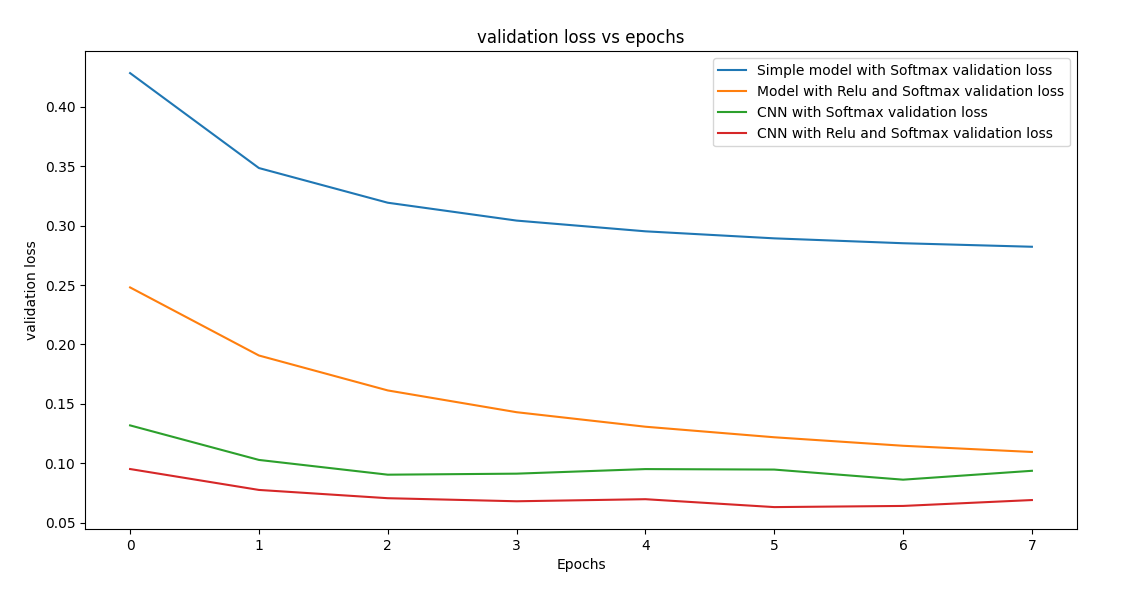
\includegraphics[width = \linewidth]{Validation_loss.png}
\end{minipage}
\smallskip

From the graph, the CNN with ReLU optimizer has the fastest convergence of training and validation losses with the highest training and validation accuracies out of four models. And on the opposite side, the simple perceptron optimizer converges much slower and has the lowest training and validation accuracies.

We run the 4 models on 10000 testing images. The first model reaches an accuracy of 92.4\% with 760 wrong predictions. The second model
reaches an accuracy of 97.0\% with 303 wrong predictions. The third model reaches an accuracy of 97.6\% with 163 wrong predictions. And the fourth  model reaches an accuracy of 98.4\% with only 120 wrong predictions. There are 29 images that none of these models are able to classify correctly.

We break down the accuracies by digits and obtain the following table:
\begin{center}
\bgroup
\def\arraystretch{1.2}
\begin{tabular}{c|c|c|c|c}
\hline
$X\setminus$ accuracy & Model 1 & Model 2 & Model 3 & Model 4 \\
\hline
0 & 0.9765 & 0.9837 & 0.9612 & 0.9612 \\
\hline
1 & 0.9824 & 0.9938 & 0.9700 & 0.9700 \\
\hline
2 & 0.8866 & 0.9671 & 0.8488 & 0.8488 \\
\hline
3 & 0.9069 & 0.9842 & 0.8832 & 0.8832 \\
\hline
4 & 0.9216 & 0.9654 & 0.8961 & 0.8961 \\
\hline
5 & 0.8744 & 0.9619 & 0.8420 & 0.8420 \\
\hline
6 & 0.9562 & 0.9749 & 0.9489 & 0.9489 \\
\hline
7 & 0.9095 & 0.9475 & 0.8774 & 0.8774 \\
\hline
8 & 0.8984 & 0.9569 & 0.8460 & 0.8460 \\
\hline
9 & 0.9177 & 0.9584 & 0.8959 & 0.8959 \\
\hline
\end{tabular}
\egroup
\end{center}
\medskip

All models had an easy time classifying numbers 0, 1, and 6. They seem to relatively struggle with predicting numbers $2$, $5$, and $8$. The perceptron with ReLU performed exceptionally well at detecting number 3 comparing to the accuracies of other models. But the overall performances of the third and the fourth models are better than the first two.
To analyze the weakness of each model, we provide a few wrongly classified images from the test set.

The following figure shows 9 images that are misclassified by all models:

\begin{minipage}{0.8\linewidth}
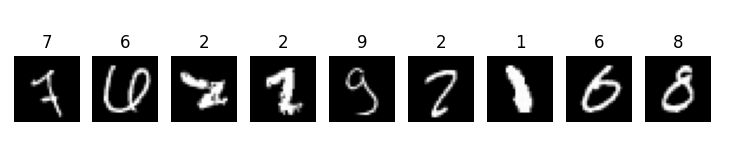
\includegraphics[width = \linewidth]{W.png}
\end{minipage}

In the following, the upper left figure shows 5 images that are misclassified by the first model, but are correctly classified by other models. The upper right figure shows 5 images that are only misclassified by the second model. Similarly, the lower left figure shows 5 images that are only misclassified by the third model. The lower right figure shows 5 images that are only misclassified by the last model.

\hspace{-0.3in}
\begin{minipage}{0.52\linewidth}
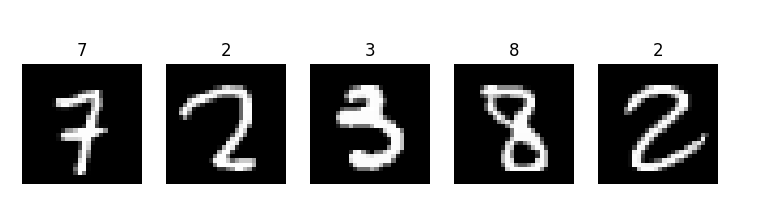
\includegraphics[width = \linewidth]{A1.png}
\end{minipage}
\begin{minipage}{0.52\linewidth}
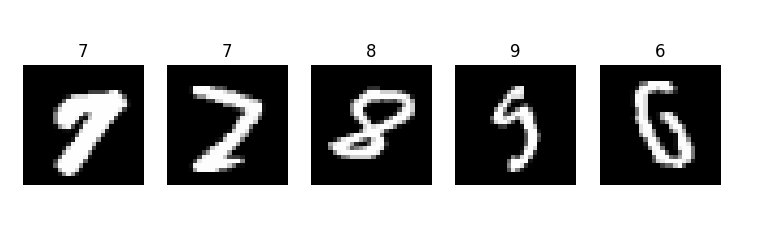
\includegraphics[width = \linewidth]{B1.png}
\end{minipage}

\hspace{-0.3in}
\begin{minipage}{0.52\linewidth}
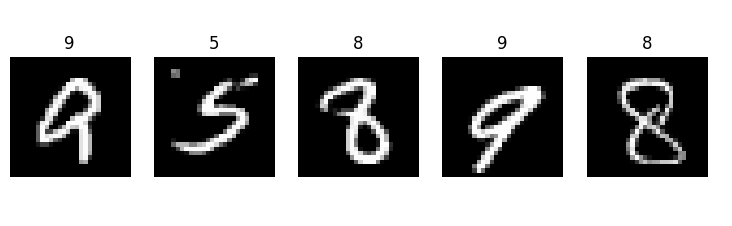
\includegraphics[width = \linewidth]{C1.png}
\end{minipage}
\begin{minipage}{0.52\linewidth}
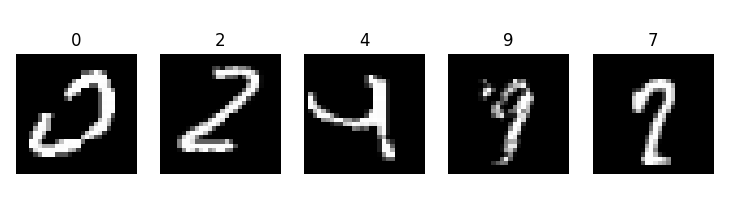
\includegraphics[width = \linewidth]{D1.png}
\end{minipage}

We observe some patterns in the kinds of features that each of the models tend to struggle with. For example, the simple perceptron can handle some discontinuous figures, but is not as good at distinguishing between curved numbers such as 2, 3, 5, and 8, even when these numbers are well written. Both of the CNNs perform noticeably better than their perceptron counterparts when classifying heavily distorted numbers caused by bad handwriting. All of the models have some level of trouble recognizing discontinuous numbers (numbers missing some parts or disconnected at some places). Adding a ReLU function helps a lot, but it does not completely solve this problem.

\section{Finding Confidence Levels}

We have seen that the four models respectively reach an accuracy of 92.4\%, 97.0\%, 97.6\%, and 98.4\% on testing images. In this section, we will use the Bayesian method to find the confidence levels of each model after predicting a certain value.
We first run all models on 10000 testing images and obtain the following four confusion matrices:

\hspace{-0.3in}
\begin{minipage}{0.5\linewidth}
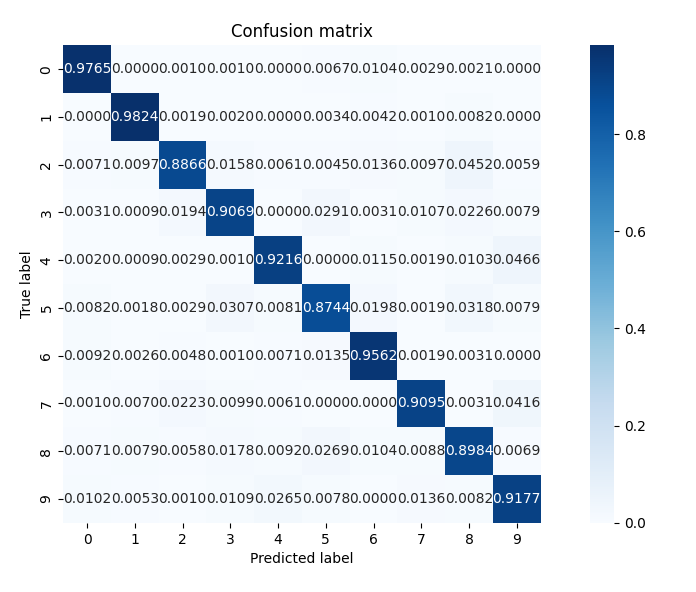
\includegraphics[width = \linewidth]{Confusion_matrix1.png}
\end{minipage}
\begin{minipage}{0.5\linewidth}
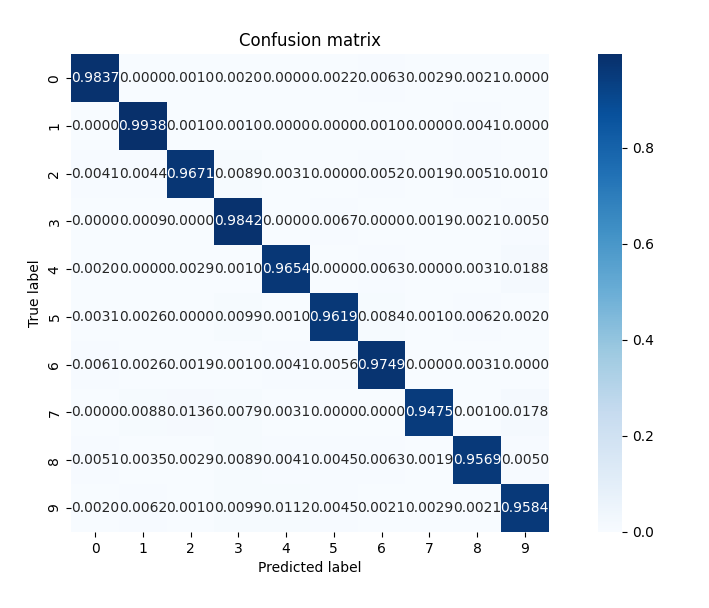
\includegraphics[width = \linewidth]{Confusion_matrix2.png}
\end{minipage}

\hspace{-0.3in}
\begin{minipage}{0.5\linewidth}
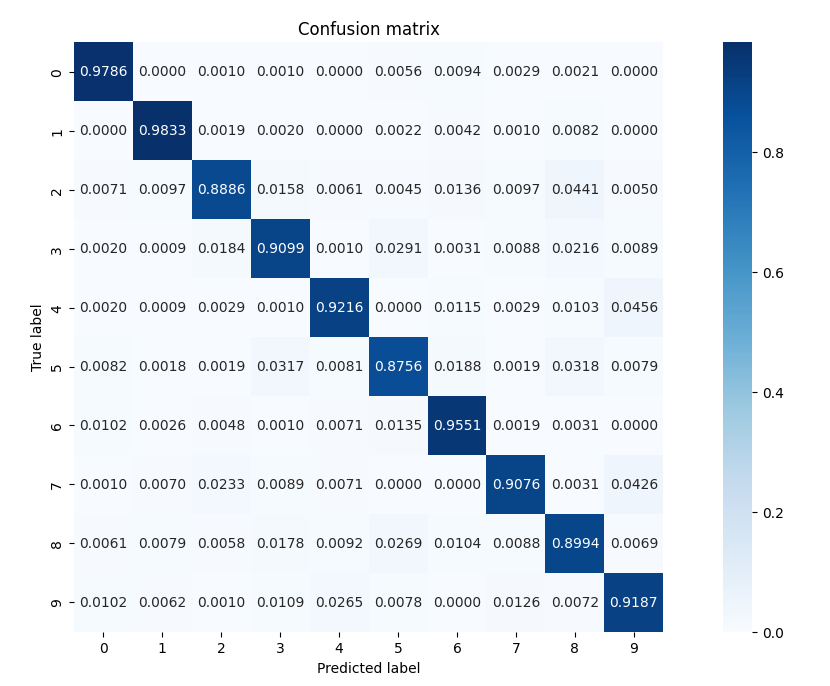
\includegraphics[width = \linewidth]{Confusion_matrix3.png}
\end{minipage}
\begin{minipage}{0.5\linewidth}
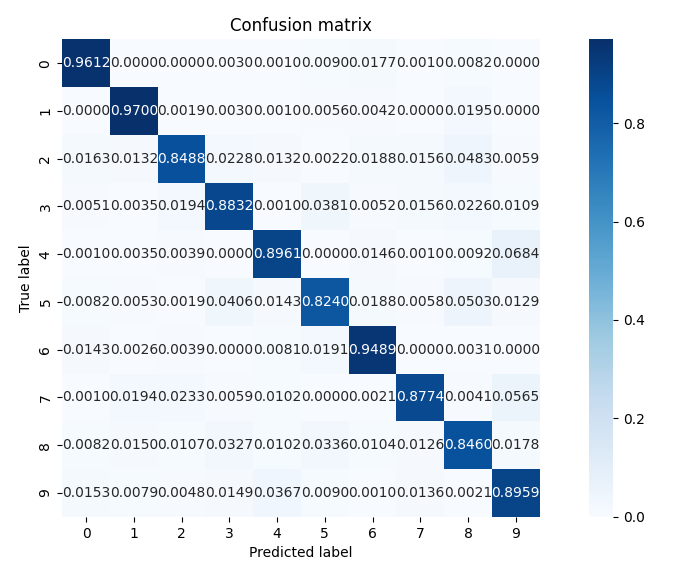
\includegraphics[width = \linewidth]{Confusion_matrix4.png}
\end{minipage}
\medskip

Let $i$ be the value predicted by a model when given a random number $X$ as input, where $0\leq i\leq 9$. We want to update the probability that this prediction is correct based on the received number $i$. By Bayes's rule
$$
P\left(X=i\,|\, {\rm Pred}=i\right)=\frac{P\left({\rm Pred}=i\,|\, X=i\right)P\left(X=i\right)}{P\left({\rm Pred}=i\right)}
=\frac{P\left({\rm Pred}=i\,|\, X=i\right)P\left(X=i\right)}{\sum_{j=0}^9P\left({\rm Pred}=i\,|\,X=j\right)P\left(X=j\right)}.
$$
For example, if $i=0$, from the confusion matrix of the simple perceptron model, we obtain the following conditional probabilities:
\medskip

$P\left({\rm Pred}=0\,|\,X=0\right)=0.9765 \qquad P\left({\rm Pred}=0\,|\,X=1\right)=0.0000$

$P\left({\rm Pred}=0\,|\,X=2\right)=0.0071$ \qquad $P\left({\rm Pred}=0\,|\,X=3\right)=0.0031$

$P\left({\rm Pred}=0\,|\,X=4\right)=0.0020$ \qquad $P\left({\rm Pred}=0\,|\,X=5\right)=0.0082$

$P\left({\rm Pred}=0\,|\,X=6\right)=0.0092$ \qquad $P\left({\rm Pred}=0\,|\,X=7\right)=0.0010$

$P\left({\rm Pred}=0\,|\,X=8\right)=0.0071$ \qquad $P\left({\rm Pred}=0\,|\,X=9\right)=0.0102$
\medskip

To compute the probability of selecting each number at random from the MNIST dataset, we count the number of images of 0, 1, 2, 3, 4, 5, 6, 7, 8, and 9 separately in the 10000 testing images. For example, there are 980 images for 0, so the probability  $P\left(X=0\right)=0.098$. Thus, we have $P\left(X=1\right)=0.1135$,
$P\left(X=2\right)=0.1032$, $P\left(X=3\right)=0.101$, $P\left(X=4\right)=0.0982$, $P\left(X=5\right)=0.0892$,
$P\left(X=6\right)=0.0958$, $P\left(X=7\right)=0.1028$, $P\left(X=8\right)=0.0974$, and $P\left(X=9\right)=0.1009$.  Plugging into Bayes's formula, we obtain
%Among the 10000 testing images, we have 980 images for 0, 1135 images for 1, 1032 images for 2, 1010 images for 3, 982 images for 4, 892 images for 5, 958 images for 6, 1028 images for 7, 974 images for 8, 1009 images for 9.
$$
P\left(X=0\,|\, {\rm Pred}=0\right)=\frac{P\left({\rm Pred}=0\,|\, X=0\right)P\left(X=0\right)}{\sum_{j=0}^9P\left({\rm Pred}=0\,|\,X=j\right)P\left(X=j\right)}
=\frac{0.0957}{0.1004}=0.9534.
$$

Thus we obtain the following updated confidence levels based on the predicted values:

\begin{center}
\bgroup
\def\arraystretch{1.2}
\begin{tabular}{c|cc|cc|cc|cc}
\hline
$X\setminus$ accuracy & Model 1 &       & Model 2 &       & Model 3 &       & Model 4 &    \\
                      & Prior  & Posterior & Prior  & Posterior & Prior  & Posterior & Prior  & Posterior \\
\hline
0 & 0.9765 & {\bf 0.9534} & 0.9837 & {\bf 0.9779} & 0.9612 & {\bf 0.9546} & 0.9612 & {\bf 0.9323}\\
\hline
1 & 0.9824 & {\bf 0.9686} & 0.9938 & {\bf 0.9750} & 0.9700 & {\bf 0.9679} & 0.9700 &  {\bf 0.9399}\\
\hline
2 & 0.8866 & {\bf 0.9362} & 0.9671 & {\bf 0.9759} & 0.8488 & {\bf 0.9372} & 0.8488 &  {\bf 0.9258}\\
\hline
3 & 0.9069 & {\bf 0.9129} & 0.9842 & {\bf 0.9523} & 0.8832 & {\bf 0.9133} & 0.8832 &  {\bf 0.8823}\\
\hline
4 & 0.9216 & {\bf 0.9356} & 0.9654 & {\bf 0.9728} & 0.8961 & {\bf 0.9336} & 0.8961 &  {\bf 0.9028}\\
\hline
5 & 0.8744 & {\bf 0.8950} & 0.9619 & {\bf 0.9737} & 0.8420 & {\bf 0.8977} & 0.8420 &  {\bf 0.8637}\\
\hline
6 & 0.9562 & {\bf 0.9278} & 0.9749 & {\bf 0.9643} & 0.9489 & {\bf 0.9296} & 0.9489 &  {\bf 0.9088}\\
\hline
7 & 0.9095 & {\bf 0.9469} & 0.9475 & {\bf 0.9874} & 0.8774 & {\bf 0.9486} & 0.8774 &  {\bf 0.9328}\\
\hline
8 & 0.8984 & {\bf 0.8674} & 0.9569 & {\bf 0.9700} & 0.8460 & {\bf 0.8703} & 0.8460 &  {\bf 0.8323}\\
\hline
9 & 0.9177 & {\bf 0.8884} & 0.9569 & {\bf 0.9513} & 0.8460 & {\bf 0.8884} & 0.8460 &  {\bf 0.8408}\\
\hline
\end{tabular}
\egroup
\end{center}
\bigskip

From the table, we see that if the model gives us the predicted values 0, 1, or 6, the confidence level for the prediction is less that the model's accuracy rate for a random image with that value as the label. If the model gives us the predicted values 2, 4, 5, or 7, we are more confident that the prediction is true than the model's accuracy rate for those numbers.

\section{Conclusion}

In this project, we trained a simple perceptron, a perceptron with a ReLU function, a perceptron with CNN, and a perceptron with both CNN and ReLU function on the MNIST dataset to classify handwritten digits. Our model can achieve test accuracies of 92.4\%, 97.0\%, 97.6\%, and 98.4\% respectively. The recognition accuracy of the combined neural network is substantially better than that of a simple perceptron. We believe the performance can be improved further when we add more convolutional layers and ReLU functions.

The experiment results show that each model struggles with some types of features more than others. This is quite common in many multiclass classification problems. We also plot a confusion matrix for each model's predictions and its corresponding true labels to gather more class-level insights. Finally, we use Baysian analysis to calculate how confident each model is with their predictions.

\section*{References}
\small

%[1] Alexander, J.A.\ \& Mozer, M.C.\ (1995) Template-based algorithms for
%connectionist rule extraction. In G.\ Tesauro, D.S.\ Touretzky and T.K.\ Leen
%(eds.), {\it Advances in Neural Information Processing Systems 7},
%pp.\ 609--616. Cambridge, MA: MIT Press.
%
%[2] Bower, J.M.\ \& Beeman, D.\ (1995) {\it The Book of GENESIS: Exploring
%  Realistic Neural Models with the GEneral NEural SImulation System.}  New York:
%TELOS/Springer--Verlag.
%
%[3] Hasselmo, M.E., Schnell, E.\ \& Barkai, E.\ (1995) Dynamics of learning and
%recall at excitatory recurrent synapses and cholinergic modulation in rat
%hippocampal region CA3. {\it Journal of Neuroscience} {\bf 15}(7):5249-5262.


[1] A. Baldominos, Y. Saez, and P. Isasi, ``A Survey of Handwritten Character Recognition with MNIST and EMNIST," vol. 9(15), Appl. Sci. 2019,  https://doi.org/10.3390/app9153169.

[2] D. C. Cire\c{s}an, U. Meier, L. M. Gambardella, J. Schmidhuber, ``Deep Big Multilayer Perceptrons for Digit Recognition," In: Montavon, G., Orr, G. B., M\"{u}ller, KR. (eds) Neural Networks: Tricks of the Trade, Lecture Notes in Computer Science, vol 7700, Springer, Berlin, Heidelberg, 2012, https://doi.org/10.1007/978-3-642-35289-8$\_$31.

[3] K. Dasgaonkar and S. Chopade, ``Analysis of multi-layered perceptron, radial basis function and convolutional neural networks in recognizing handwritten digits," International Journal of Advance Research, Ideas and Innovations in Technology, vol. 4, 2018, page 2429-2431.

[4] Y. LeCun, C. Cortes, and C. J. Burges, ``MNIST handwritten digit database," ATT Labs (Online), http://yann.lecun.com/exdb/mnist, vol. 2, 2010.

[5] Y. Hou and H. Zhao, ``Handwritten digit recognition based on depth neural network," 2017 International Conference on Intelligent Informatics and Biomedical Sciences (ICIIBMS), 2017, doi: 10.1109/ICIIBMS.2017.8279710.

\end{document}
